\documentclass[12pt,a4paper]{article}

\usepackage[T1]{fontenc}
\usepackage[utf8]{inputenc}
\usepackage{lmodern}
\usepackage{microtype}
\usepackage[a4paper,margin=2.54cm]{geometry}
\usepackage{amsmath,amssymb}
\usepackage{array}
\usepackage{xcolor}
\usepackage{booktabs}
\usepackage{setspace}
\usepackage[hidelinks]{hyperref}
\usepackage{tikz}
\usetikzlibrary{positioning,arrows.meta,shapes.geometric,fit,backgrounds}

\setlength{\parindent}{1.5em}
\setlength{\parskip}{0pt}
\setlength{\emergencystretch}{2em}
\newcolumntype{P}[1]{>{\raggedright\arraybackslash}p{#1}}

\begin{document}

\begin{center}
    {\Large\bfseries
    Structure-Resolved Hybrid Modelling of CO$_2$ Adsorption in\par
    DEM-Generated Packed Beds\par}
    \vspace{1.25em}
    {\normalsize Ali Khalifa and Heba Alzaben\par}
    \vspace{0.6em}
    {\small Technical University of Munich, Freising, Germany;\par
    Al Hussein Technical University, Amman, Jordan\par}
\end{center}

\vspace{1.25em}
\setstretch{1.5}

\begin{abstract}
Packed-bed adsorption depends on sorbent chemistry and on the void pathways
through which gas reaches the particles. Beds with nearly equal bulk porosity
can therefore exhibit different transient utilization. This study develops an
isothermal framework containing no CFD. The discrete-element method generates
twenty mechanically realizable beds of monodisperse commercial zeolite 13X
beads. A geometry-defined pore network is extracted from each packing, and a
conservative transient solver couples gas-phase CO$_2$ diffusion through pore
throats to one linear-driving-force adsorption equation per bead. All cases use
the same geometry scale, material parameters and finite-area inlet condition;
only the stochastic packing changes. At 5000~s, uptake varies from 0.206 to
0.315~mol~kg$^{-1}$ although bulk porosity occupies only a narrow range.
Porosity-only leave-one-bed-out models have negative predictive $R^2$. In
contrast, a physically defined steady conductance from the inlet to a plane
five particle diameters inside the bed correlates strongly with uptake
($\rho=0.968$) and underutilized-particle fraction ($\rho=-0.959$). The number
of distinct second-layer pores is most closely associated with the relative
half-uptake time ($\rho=-0.814$). The current paper therefore focuses on
interpretable inlet accessibility and internal transport rather than graph
neural networks. A homogeneous one-dimensional model reproduces the twenty
network uptake curves with a mean time-weighted NRMSE of 1.58\% when one
effective diffusivity is fitted per bed. Those diffusivities vary by 23.1\%,
despite a bulk-porosity coefficient of variation near 0.55\%. A positive
accessibility-based power law predicts withheld-bed diffusivity with
$R^2=0.890$, whereas porosity alone gives $R^2=-0.234$. The contribution is a
reproducible DEM--pore-network--homogeneous route and an interpretable closure
showing which structural information bulk porosity misses.
\end{abstract}

\noindent\textbf{Keywords:} carbon dioxide adsorption; zeolite 13X; packed bed;
discrete-element method; pore network; inlet accessibility; hybrid modelling;
linear driving force

\section{Motivation, research gap and hypothesis}

Fixed beds of porous adsorbent particles are widely considered for CO$_2$
separation. At the material scale, equilibrium capacity and intracrystalline or
macropore transport determine how much and how rapidly CO$_2$ can be stored. At
the bed scale, the arrangement of the beads determines the connected void space
through which CO$_2$ reaches the sorbent. Standard column models average the
second contribution into a bed porosity, an axial-dispersion coefficient and an
effective kinetic constant. This is efficient but cannot distinguish two beds
with equal global descriptors and different local bottlenecks.

Particle-resolved flow simulations could resolve this heterogeneity, but they
would dominate the cost of producing hundreds of independent packings. The
present proposal instead uses a geometry-defined transport network. Pore-network
models replace the continuous void phase by pore bodies connected by throats and
can enforce local conservation at much lower cost than a resolved continuum
calculation \cite{Blunt2017}. The network is not an arbitrary graph: its nodes,
edges, lengths and cross-sections are extracted from a mechanically realizable
DEM packing.

The present reduction uses transparent physical descriptors rather than a
learned graph representation. It identifies structural information that is
lost when a packing is reduced to porosity or mean particle size and expresses
that information through a small number of closure variables for a cheaper
model. The central hypothesis is:

\begin{quote}
For DEM beds with matched particle-size distribution and global porosity,
diffusion-limited CO$_2$ uptake still varies because of differences in inlet
accessibility, pore connectivity and throat bottlenecks. A physically defined
inlet-to-interior conductance and a small number of spatial descriptors capture
this variation more reliably than global porosity alone.
\end{quote}

This hypothesis is falsifiable. The proposed descriptors are unnecessary if
porosity and a conventional tortuosity estimate predict withheld beds with
comparable accuracy. Models are therefore compared by leaving out one complete
packing at a time, not by reporting training accuracy.

\section{Scope and physical interpretation}

The recommended first paper addresses an initially CO$_2$-free, nitrogen-filled
bed exposed to a prescribed CO$_2$ concentration at its lower boundary. CO$_2$
penetrates the initially stagnant gas by diffusion and is adsorbed by the beads.
The upper boundary is closed or assigned a specified concentration depending on
the verification test. There is no imposed gas velocity, Navier--Stokes solver
or CFD component. Consequently, the principal outputs are transient uptake,
penetration depth and sorbent utilization, not a flowing-column breakthrough
curve.

This restriction is important. A diffusion-only network is a defensible first
test of how packing geometry influences transport and adsorption. It must not
be described as a complete pressure- or vacuum-swing adsorption column model.
A later extension can add a pressure-resistance network and throat advection,
still without CFD, but that extension should follow validation of the present
diffusion--adsorption solver.

Figure~\ref{fig:problem} illustrates the physical problem and the two coupled
graphs. DEM particles define the solid skeleton. The dual pore network carries
gas-phase CO$_2$, while every adsorbing particle retains its own solid loading.

\begin{figure}[!htbp]
\centering
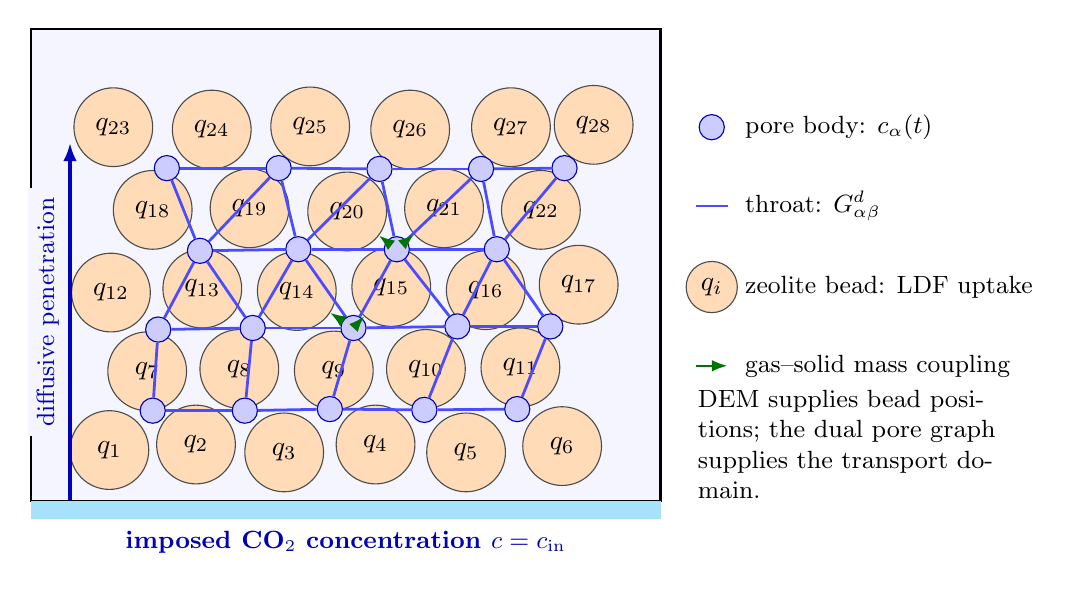
\begin{tikzpicture}[
 bead/.style={circle,draw=black!70,fill=orange!28,minimum size=10mm,inner sep=0pt},
 pore/.style={circle,draw=blue!70!black,fill=blue!20,minimum size=3.2mm,inner sep=0pt},
 throat/.style={draw=blue!70,line width=1.0pt},
 uptake/.style={-{Latex[length=2mm]},green!45!black,line width=0.85pt},
 diff/.style={-{Latex[length=2.3mm]},blue!75!black,very thick},
 lab/.style={font=\small,align=left}
]
\fill[blue!4] (0,0) rectangle (8,6);
\draw[thick] (0,0) rectangle (8,6);
\fill[cyan!35] (0,-0.22) rectangle (8,0);
\node[font=\small\bfseries,blue!70!black] at (4,-0.52)
      {imposed CO$_2$ concentration $c=c_{\mathrm{in}}$};

\node[bead] (b1) at (1.0,0.65) {$q_1$};
\node[bead] (b2) at (2.1,0.72) {$q_2$};
\node[bead] (b3) at (3.22,0.62) {$q_3$};
\node[bead] (b4) at (4.38,0.72) {$q_4$};
\node[bead] (b5) at (5.53,0.62) {$q_5$};
\node[bead] (b6) at (6.75,0.70) {$q_6$};
\node[bead] (b7) at (1.48,1.65) {$q_7$};
\node[bead] (b8) at (2.65,1.68) {$q_8$};
\node[bead] (b9) at (3.85,1.66) {$q_9$};
\node[bead] (b10) at (5.02,1.68) {$q_{10}$};
\node[bead] (b11) at (6.22,1.70) {$q_{11}$};
\node[bead] (b12) at (1.02,2.65) {$q_{12}$};
\node[bead] (b13) at (2.18,2.70) {$q_{13}$};
\node[bead] (b14) at (3.38,2.67) {$q_{14}$};
\node[bead] (b15) at (4.58,2.72) {$q_{15}$};
\node[bead] (b16) at (5.78,2.68) {$q_{16}$};
\node[bead] (b17) at (6.96,2.75) {$q_{17}$};
\node[bead] (b18) at (1.55,3.70) {$q_{18}$};
\node[bead] (b19) at (2.78,3.72) {$q_{19}$};
\node[bead] (b20) at (4.02,3.68) {$q_{20}$};
\node[bead] (b21) at (5.25,3.72) {$q_{21}$};
\node[bead] (b22) at (6.48,3.70) {$q_{22}$};
\node[bead] (b23) at (1.05,4.75) {$q_{23}$};
\node[bead] (b24) at (2.30,4.72) {$q_{24}$};
\node[bead] (b25) at (3.55,4.76) {$q_{25}$};
\node[bead] (b26) at (4.82,4.72) {$q_{26}$};
\node[bead] (b27) at (6.10,4.75) {$q_{27}$};
\node[bead] (b28) at (7.15,4.78) {$q_{28}$};

\node[pore] (p1) at (1.55,1.15) {};
\node[pore] (p2) at (2.72,1.15) {};
\node[pore] (p3) at (3.80,1.17) {};
\node[pore] (p4) at (5.00,1.16) {};
\node[pore] (p5) at (6.18,1.17) {};
\node[pore] (p6) at (1.62,2.18) {};
\node[pore] (p7) at (2.82,2.20) {};
\node[pore] (p8) at (4.10,2.20) {};
\node[pore] (p9) at (5.42,2.22) {};
\node[pore] (p10) at (6.60,2.22) {};
\node[pore] (p11) at (2.15,3.18) {};
\node[pore] (p12) at (3.40,3.20) {};
\node[pore] (p13) at (4.65,3.20) {};
\node[pore] (p14) at (5.92,3.20) {};
\node[pore] (p15) at (1.73,4.23) {};
\node[pore] (p16) at (3.15,4.23) {};
\node[pore] (p17) at (4.43,4.22) {};
\node[pore] (p18) at (5.72,4.22) {};
\node[pore] (p19) at (6.78,4.23) {};

\foreach \a/\b in {p1/p2,p2/p3,p3/p4,p4/p5,p1/p6,p2/p7,p3/p8,p4/p9,p5/p10,
 p6/p7,p7/p8,p8/p9,p9/p10,p6/p11,p7/p11,p7/p12,p8/p12,p8/p13,p9/p13,p9/p14,
 p10/p14,p11/p12,p12/p13,p13/p14,p11/p15,p11/p16,p12/p16,p12/p17,p13/p17,
 p13/p18,p14/p18,p14/p19,p15/p16,p16/p17,p17/p18,p18/p19}
 \draw[throat] (\a)--(\b);

\draw[diff] (0.50,0.02)--(0.50,4.55);
\node[lab,rotate=90,blue!75!black,fill=blue!4] at (0.22,2.40)
      {diffusive penetration};
\draw[uptake] (p8)--(b14);
\draw[uptake] (p8)--(b15);
\draw[uptake] (p13)--(b20);
\draw[uptake] (p13)--(b21);

\node[pore] at (8.65,4.75) {};
\node[lab,anchor=west] at (8.95,4.75) {pore body: $c_\alpha(t)$};
\draw[throat] (8.45,3.75)--(8.85,3.75);
\node[lab,anchor=west] at (8.95,3.75) {throat: $G_{\alpha\beta}^{d}$};
\node[bead,minimum size=6.5mm] at (8.65,2.72) {$q_i$};
\node[lab,anchor=west] at (8.95,2.72) {zeolite bead: LDF uptake};
\draw[uptake] (8.45,1.72)--(8.85,1.72);
\node[lab,anchor=west] at (8.95,1.72) {gas--solid mass coupling};
\node[lab,anchor=west,text width=4.0cm] at (8.35,0.72)
      {DEM supplies bead positions; the dual pore graph supplies the transport domain.};
\end{tikzpicture}
\caption{Schematic of the proposed diffusion--adsorption problem. Gas-phase
CO$_2$ concentrations $c_\alpha$ are solved on pore bodies connected by
geometry-derived throat conductances. Each zeolite bead has a separate loading
$q_i$ governed by an LDF equation. Gas removed by adsorption appears with equal
and opposite sign in the neighboring pore balances.}
\label{fig:problem}
\end{figure}

\section{Choice of sorbent and model parameters}

\subsection{Why zeolite 13X is the recommended first material}

Commercial zeolite 13X is selected for four reasons. First, it is a benchmark
physical adsorbent for post-combustion CO$_2$ separation and exhibits strong
CO$_2$/N$_2$ selectivity \cite{Dantas2011,Hu2014}. Second, commercial 13X is
available as nearly spherical millimetre-scale beads, making the relationship
between the laboratory material and a spherical DEM representation unusually
direct. Hu et al. studied commercial beads with radii of approximately 0.8,
0.98 and 1.95~mm and found that CO$_2$ uptake under representative conditions
was governed primarily by macropore diffusion \cite{Hu2014}. This supports the
use of a bead-scale LDF kinetic law. Third, equilibrium and transient data are
available for checking the adsorption submodel. Dantas et al. demonstrated
that a Toth equilibrium model combined with LDF kinetics can reproduce CO$_2$
and CO$_2$/N$_2$ fixed-bed adsorption on 13X \cite{Dantas2011}. Fourth, using a
single established sorbent isolates the proposed contribution: the influence
of bed geometry, rather than a comparison of sorbent chemistries.

Activated carbon is not chosen for the pilot because its surface chemistry and
pore-size distributions vary strongly between feedstocks and activation
routes. Amine-functionalized solids and reactive pellets are also postponed
because humidity sensitivity, reaction kinetics and thermal effects would make
it difficult to identify whether an observed trend comes from bed structure or
material chemistry.

\subsection{Reference properties and their status}

Table~\ref{tab:parameters} distinguishes physical inputs from numerical DEM
choices. This distinction is essential. The density, bead size and adsorption
data should correspond to a selected commercial 13X dataset. By contrast, the
DEM Young's modulus may be reduced to increase the stable timestep, provided
the maximum overlap and final packing statistics are shown to be insensitive
to further stiffness increases.

\begin{table}[!htbp]
\centering
\caption{Proposed baseline properties for the first study. Adsorption
parameters are fitted as one internally consistent set to a chosen 13X
isotherm/uptake dataset; values from different products are not mixed.}
\label{tab:parameters}
\scriptsize
\renewcommand{\arraystretch}{0.88}
\begin{tabular}{P{3.25cm}P{3.1cm}P{6.45cm}}
\toprule
\textbf{Quantity} & \textbf{Baseline/range} & \textbf{Choice and justification} \\
\midrule
Sorbent & commercial zeolite 13X & benchmark CO$_2$ adsorbent; strong CO$_2$/N$_2$ selectivity; documented bead-scale kinetics \\
Bead diameter & 1.6~mm baseline; 1.4--2.0~mm sensitivity & 1.6~mm corresponds to the commercial $R\approx0.8$~mm bead studied by Hu et al.; a narrow range tests polydispersity without changing material \\
Particle shape & sphere & consistent with approximately spherical commercial beads and provides an unambiguous radical-Voronoi pore construction \\
Apparent bead density & approximately $1.6\times10^3$~kg,m$^{-3}$, verified for the selected batch & consistent with the reported 3.5~mg mass and 0.8~mm radius as an approximate inference; final simulations should use directly reported or measured batch data \\
Solid density for adsorption conversion & 1950~kg,m$^{-3}$ where the Dantas dataset is used & reported for the 13X sorbent in the selected fixed-bed study; it must not be silently interchanged with apparent bulk-bed density \\
Poisson ratio & 0.25 & representative numerical value for a brittle porous bead; low influence on the final gravity-packed geometry \\
DEM Young's modulus & $10^8$~Pa baseline; $10^7$--$10^9$~Pa sensitivity & intentionally softened numerical stiffness; accepted only when normalized overlaps and packing descriptors are stiffness independent \\
Particle friction & 0.4 baseline; 0.2--0.6 sensitivity & spans plausible smooth-to-rough granular packing behaviour and generates controlled structural variability \\
Restitution coefficient & 0.3 & promotes rapid settling; it affects the preparation transient rather than the static adsorption equations \\
Rolling-friction coefficient & 0.02 baseline; 0--0.05 sensitivity & represents resistance caused by bead roughness and nonsphericity not resolved by perfect spheres \\
Temperature & 311~K baseline & matches the 38$^\circ$C kinetic condition reported by Hu et al.; the first network model is isothermal \\
Feed CO$_2$ partial pressure & 0.1~bar & representative dilute post-combustion condition used in the single-bead kinetic experiments \\
Intrabead porosity and tortuosity & product-specific; e.g. $\varepsilon_p=0.269$, $\tau_p=2.61$ for $R=0.98$~mm & independently characterized values reported by Hu et al.; used for a diffusion-based check of the fitted LDF coefficient \\
Equilibrium model & Toth reference; Langmuir baseline comparison & Toth was validated for 13X over a broad temperature range; Langmuir provides a transparent low-pressure comparison \\
Kinetic coefficient & $k_{\mathrm{LDF}}$ fitted or calculated consistently for the selected bead and gas & depends on bead radius, macropore diffusivity, temperature and carrier gas and must therefore not be treated as a universal material constant \\
\bottomrule
\end{tabular}
\end{table}

The baseline bed should contain approximately 1000--3000 particles. Smaller
200--500 particle beds are useful for debugging, mesh and exact-conservation
tests, but can exaggerate boundary effects. Cylinder-to-particle diameter ratios
of 10, 15 and 20 are proposed so that wall-induced packing structure can be
quantified. A bed-height-to-diameter ratio of approximately 2 is sufficient for
the first diffusion-uptake problem without creating an unnecessarily large
network.

\section{Hybrid modelling concept}

\subsection{DEM packing generation}

Spherical beads are inserted above a cylindrical container and settle under
gravity. The final state is accepted only after the kinetic energy and mean
particle velocity fall below prescribed tolerances. Independent random seeds,
wall friction and particle friction generate different mechanically realizable
structures. Particle number, size distribution and target bed dimensions are
controlled so that stochastic topology can be studied separately from bulk
porosity.

Required DEM outputs are particle centres, radii, contacts and wall contacts.
Acceptance checks include particle count, size distribution, bed height,
porosity, radial and axial porosity profiles, coordination number, maximum
normalized overlap and reproducibility. The adsorption state does not act back
on the particle motion in the first study; the geometry is frozen after packing.

\subsection{Geometry-defined pore network}

The final DEM geometry is converted to a radical-Delaunay tessellation, which
accounts for unequal sphere radii. The dual weighted Voronoi cells define pore
bodies and their shared faces define candidate throats. Each pore body
$\alpha$ has gas volume $V_\alpha$, and each throat $\alpha\beta$ has length
$L_{\alpha\beta}$ and open cross-sectional area $A_{\alpha\beta}$. The initial
diffusive conductance is
\begin{equation}
 G_{\alpha\beta}^{d}
 =D_{\mathrm{CO_2,N_2}}
  \frac{A_{\alpha\beta}}{L_{\alpha\beta}},
 \label{eq:diffconductance}
\end{equation}
where $D_{\mathrm{CO_2,N_2}}$ is the binary molecular diffusivity. An optional
shape factor can be introduced only after comparison with simple analytical
geometries. Unlike a proximity cutoff chosen by hand, this construction derives
network connectivity from the void geometry.

\subsection{Where and how adsorption is implemented}

Adsorption is implemented in the transient pore-network solver, not in DEM and
not inside a data-driven surrogate. DEM ends after producing the fixed geometry. Each physical
bead $i$ receives a time-dependent average solid loading $q_i(t)$ in
mol,kg$^{-1}$. The local gas concentration seen by the bead is the
area-weighted concentration of its adjacent pores,
\begin{equation}
 c_i^{g}=\frac{\sum_{\alpha\in\mathcal P_i}
 A_{i\alpha}c_\alpha}
 {\sum_{\alpha\in\mathcal P_i}A_{i\alpha}},
 \label{eq:localconcentration}
\end{equation}
where $\mathcal P_i$ contains the pore bodies adjacent to particle $i$ and
$A_{i\alpha}$ is the particle surface area associated with pore $\alpha$.

For the transparent baseline, the equilibrium loading follows a Langmuir law,
\begin{equation}
 q_i^*=\frac{q_{\max}b(T)p_i}
 {1+b(T)p_i}, \qquad p_i=c_i^gRT.
 \label{eq:langmuir}
\end{equation}
The primary model uses the Toth isotherm fitted to the selected 13X data,
\begin{equation}
 q_i^*=\frac{q_m b p_i}
 {\left[1+(b p_i)^n\right]^{1/n}}.
 \label{eq:toth}
\end{equation}
The bead-average uptake is governed by the LDF equation
\begin{equation}
 \frac{dq_i}{dt}=k_{\mathrm{LDF},i}
 \left(q_i^*-q_i\right).
 \label{eq:ldf}
\end{equation}
For macropore-diffusion control, the fitted coefficient is checked against the
spherical-particle estimate
\begin{equation}
 k_{\mathrm{LDF},i}\approx
 \frac{15D_{e,i}}{R_i^2},
 \label{eq:ldfcheck}
\end{equation}
with the precise coefficient and effective diffusivity definition kept
consistent with the selected LDF derivation.

The conservative gas balance for every pore body is
\begin{equation}
 V_\alpha\frac{dc_\alpha}{dt}
 =\sum_{\beta\in\mathcal N_\alpha}
 G_{\alpha\beta}^{d}(c_\beta-c_\alpha)
 -\sum_{i\in\mathcal S_\alpha}
 w_{i\alpha}m_i\frac{dq_i}{dt},
 \label{eq:porebalance}
\end{equation}
where $m_i$ is dry sorbent mass and
$w_{i\alpha}=A_{i\alpha}/\sum_{\gamma\in\mathcal P_i}A_{i\gamma}$ distributes
the bead uptake among its neighboring pores. The same adsorption rate added to
the solid in Eq.~\eqref{eq:ldf} is removed from the gas in
Eq.~\eqref{eq:porebalance}. Thus, total CO$_2$ is conserved to time-integration
tolerance.

The coupled ODE system is stiff when throat conductances and adsorption rates
span wide ranges. An implicit BDF or backward-Euler method with adaptive time
stepping is therefore recommended. At every step the implementation evaluates
local concentrations, equilibrium loadings, LDF rates and pore sinks as one
coupled residual. Sequentially updating adsorption after gas diffusion would be
allowed only after a timestep-convergence study.

\subsection{Reference outputs}

Each network simulation provides:
\begin{itemize}
 \item total uptake $M_{\mathrm{ads}}(t)=\sum_i m_iq_i(t)$;
 \item times $t_{50}$ and $t_{90}$ to reach 50 and 90\% of final uptake;
 \item axial penetration and loading profiles;
 \item particle-level utilization $q_i/q_i^*$;
 \item poorly utilized fraction at a prescribed time;
 \item effective bed diffusivity from a separate non-adsorbing steady test;
 \item mass-balance error and boundary CO$_2$ flux.
\end{itemize}

The effective diffusivity is obtained by imposing concentrations $c_{\mathrm h}$
and $c_{\mathrm l}$ at opposite bed boundaries, solving the non-adsorbing steady
network, and calculating
\begin{equation}
 D_{\mathrm{eff}}=
 \frac{\dot N_{\mathrm{CO_2}}H}
 {A(c_{\mathrm h}-c_{\mathrm l})}.
 \label{eq:deff}
\end{equation}
This test separates pure bed transport from adsorption kinetics.

\subsection{Physical accessibility descriptors and homogeneous reduction}

For a throat $ij$, the diffusive conductance is
\begin{equation}
 G_{ij}=D\frac{A_{ij}}{L_{ij}}.
\end{equation}
An effective inlet-to-interior conductance $G_{\mathrm{in,int}}$ is calculated
without adsorption by fixing the inlet-pore concentration to one and the
concentration of pores at least five particle diameters into the bed to zero.
Conservation is solved at all intermediate pores, and the total inlet flux for
this unit concentration difference defines $G_{\mathrm{in,int}}$. Additional
descriptors measure unique second-layer pores, inlet-to-interior throat count,
polar coverage, inlet pore volume and geometric tortuosity.

Initial results across the twenty accepted beds show that bulk porosity is not
predictive, whereas $G_{\mathrm{in,int}}$ has Spearman correlations of 0.968
with uptake at 5000~s and -0.959 with the underutilized-particle fraction. The
unique second-layer pore count correlates with $t_{50}$ at -0.814. Bootstrap
intervals exclude zero and the corresponding univariate correlations remain
significant after false-discovery-rate correction. These observations motivate
predefined low-dimensional models rather than unrestricted feature selection.

The reduced leave-one-bed-out comparison confirms that one descriptor is
sufficient for each main response. Conductance alone gives $R^2=0.924$ for
uptake at 5000~s and $R^2=0.863$ for the underutilized-particle fraction.
Unique second-layer pore count gives $R^2=0.651$ for $t_{50}$. All three
target-permutation tests give $p<0.002$ with 500 permutations. Adding
tortuosity or polar coverage does not improve these parsimonious models; the
three-variable alternative raises uptake $R^2$ only to 0.931 and worsens the
underutilization prediction.

The accessibility plane was also moved to $3d_p$, $7d_p$ and $10d_p$.
Spearman rank correlations among the four conductance definitions are
0.953--0.993. Their correlations with uptake remain 0.950--0.970, while those
with the underutilized fraction remain -0.946 to -0.968. Absolute conductance
decreases with depth, as required by the increasing resistance, but the
structural ranking is preserved. The $5d_p$ definition is therefore retained
as a primary entrance-accessibility measure, with the other depths reported as
a robustness test.

The selected physical quantities will parameterize a homogeneous
one-dimensional model,
\begin{align}
 \varepsilon_b\frac{\partial c}{\partial t}
 &=D_{\mathrm{eff}}
 \frac{\partial^2c}{\partial z^2}
 -(1-\varepsilon_b)\rho_b\frac{\partial q}{\partial t},
 \label{eq:homogeneousgas}\\
 \frac{\partial q}{\partial t}
 &=k_{\mathrm{eff}}
 [q^*(c)-q].
 \label{eq:homogeneousads}
\end{align}
Here ``solving the homogeneous bed'' means solving
Eqs.~\eqref{eq:homogeneousgas}--\eqref{eq:homogeneousads} along the bed height
without individual pores or beads. Structure-dependent closure parameters are fitted to the conservative
network curves and then related to the physical accessibility descriptors. The
homogeneous prediction is compared against the complete network uptake curve,
not only against scalar targets.

The inlet is discretized as a Robin boundary. Because concentrations are stored
at cell centres, the external transfer resistance and diffusion across half of
the first cell act in series:
\begin{equation}
 J_{\mathrm{in}}=
 \frac{c_{\mathrm{res}}-c_1}
 {1/h_{\mathrm{in}}+\Delta z/(2D_{\mathrm{eff}})}.
 \label{eq:homogeneous-robin}
\end{equation}
This half-cell resistance is necessary for spatial-grid convergence. The fit
uses a time-integrated squared loading error, so logarithmically dense early
outputs do not receive disproportionate weight.

For seed 18427, corrected 100-, 200- and 400-cell fits give
$D_{\mathrm{eff}}=8.7422$, 8.7286 and $8.7252\times10^{-7}$~m$^2$~s$^{-1}$,
respectively. The corresponding time-weighted normalized RMSE values are
1.412\%, 1.423\% and 1.427\%. The diffusivity changes by only 0.156\% from 100
to 200 cells and 0.039\% from 200 to 400 cells; 100 cells are therefore used in
the campaign. The accepted test has a maximum absolute mass-balance residual
of $1.38\times10^{-13}$~mol and a final relative error of
$7.03\times10^{-11}$.

All twenty homogeneous fits passed quality checks. Their fitted effective
diffusivities range from $4.340\times10^{-7}$ to
$1.096\times10^{-6}$~m$^2$~s$^{-1}$, with mean
$7.584\times10^{-7}$~m$^2$~s$^{-1}$ and coefficient of variation 23.1\%.
The mean time-weighted fit NRMSE is 1.58\%.

An accessibility diffusivity is defined as
\begin{equation}
 D_{\mathrm{access}}=\frac{G_{\mathrm{in,int}}H}{A_{\mathrm{tube}}}.
 \label{eq:daccess}
\end{equation}
At the primary $5d_p$ depth, $D_{\mathrm{access}}$ and $D_{\mathrm{eff}}$
have Pearson correlation 0.951 and Spearman correlation 0.953. Direct
proportionality gives leave-one-bed-out $R^2=0.555$ and is too restrictive.
An affine model gives $R^2=0.881$ but has a negative intercept. The preferred
positive empirical closure is
\begin{equation}
 \frac{D_{\mathrm{eff}}}{D_m}=0.7589
 \left(\frac{D_{\mathrm{access}}}{D_m}\right)^{2.4969},
 \label{eq:closure}
\end{equation}
where $D_m=1.5\times10^{-5}$~m$^2$~s$^{-1}$. It gives
leave-one-bed-out $R^2=0.890$, and the bootstrap interval for the exponent is
2.057--2.768. Porosity alone gives $R^2=-0.234$. Equation~\eqref{eq:closure}
is internally validated for the present geometry and is not claimed as a
universal packed-bed correlation.

\section{Proposed work packages}

\subsection*{WP1: Material definition and controlled DEM ensemble}

Select one commercial 13X dataset and define bead size, density, equilibrium
and kinetic parameters consistently. Generate a small verification ensemble
followed by statistically independent beds. Vary random seed, friction,
polydispersity and cylinder-to-particle diameter ratio. Retain matched groups
with nearly equal porosity and size distribution but different topology.

\textbf{Deliverables:} accepted DEM files; parameter provenance table;
packing-quality report; particle and contact visualization.

\subsection*{WP2: Pore-network extraction and geometric verification}

Construct the radical-Delaunay/Voronoi network and calculate pore volumes,
throat areas, lengths and particle--pore surface associations. Verify total
solid and void volume, connectivity, boundary identification and convergence
with geometric tolerances. Test ordered sphere arrays and small packings with
analytically understood bottlenecks.

\textbf{Deliverables:} reproducible DEM-to-network converter; pore/throat files;
geometry verification cases.

\subsection*{WP3: Conservative diffusion--adsorption solver}

Implement Eqs.~\eqref{eq:ldf} and \eqref{eq:porebalance}. Begin with
non-adsorbing diffusion, then equilibrium adsorption, and finally transient LDF
kinetics. Verify mass conservation, positivity, equilibrium capacity,
timestep convergence and expected scaling with bed height, molecular
diffusivity and bead radius.

\textbf{Deliverables:} transient solver; verification report; particle and pore
uptake histories; effective-diffusivity and uptake labels.

\subsection*{WP4: Structural mechanisms and conventional baselines}

Quantify how uptake, $t_{50}$ and poorly utilized fraction vary between matched
packings. Compare porosity with inlet-to-interior conductance, second-layer
pathways, polar coverage, tortuosity and throat statistics. Use bootstrap
intervals, leave-one-bed-out prediction and target-permutation tests. Determine
whether the response reflects physical accessibility rather than global
porosity or a boundary-labelling artifact.

\textbf{Deliverables:} structure--performance database; baseline models;
matched-packing analysis; physical interpretation of bottlenecks.

\subsection*{WP5: Homogeneous model and physical closure}

Solve Eqs.~\eqref{eq:homogeneousgas}--\eqref{eq:homogeneousads} with the same bed
height, inlet concentration, isotherm, LDF coefficient and initial condition as
the pore-network cases. Fit an effective transport closure separately to each
reference curve. Test whether porosity alone predicts that closure and whether
inlet-to-interior conductance, second-layer connectivity and polar coverage
provide a reproducible improvement on withheld beds.

\textbf{Deliverables:} verified one-dimensional solver; fitted closure values;
out-of-fold physical correlations; full-curve comparison and timing analysis.

\subsection*{WP6: Robustness and publication decision}

Repeat the analysis for an unseen bead-size distribution and bed diameter.
Quantify uncertainty across seeds and sensitivity to throat definitions, inlet
labelling and the chosen five-particle-diameter accessibility depth. Repeat a
limited set at another diameter ratio if resources permit. Graph learning is
reserved for later work and is considered only after a substantially larger
geometry ensemble exists and transparent closures have been exhausted.

Figure~\ref{fig:workflow} summarizes the work-package dependencies.

\begin{figure}[!htbp]
\centering
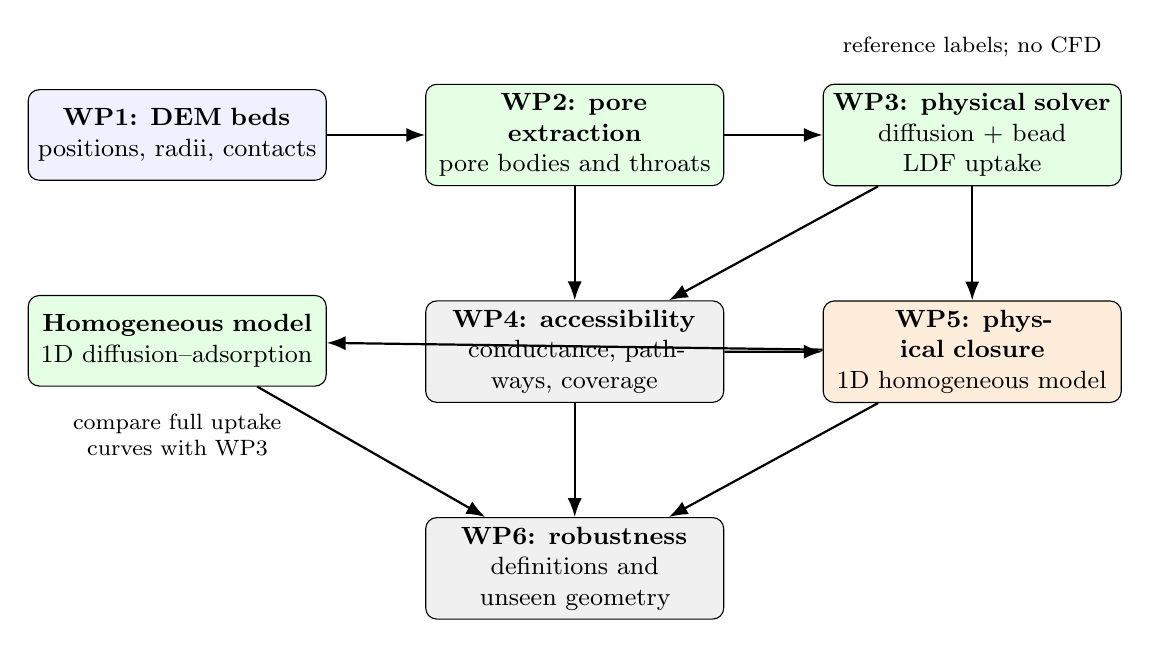
\begin{tikzpicture}[
 box/.style={draw,rounded corners,align=center,text width=3.55cm,minimum height=1.15cm,
             fill=blue!6,font=\small},
 phys/.style={box,fill=green!10},
 ml/.style={box,fill=orange!14},
 check/.style={box,fill=gray!12},
 arr/.style={-{Latex[length=2.4mm]},thick},
 note/.style={font=\footnotesize,align=center,text width=3.4cm}
]
\node[box] (wp1) {\textbf{WP1: DEM beds}\\positions, radii, contacts};
\node[phys,right=1.25cm of wp1] (wp2) {\textbf{WP2: pore extraction}\\pore bodies and throats};
\node[phys,right=1.25cm of wp2] (wp3) {\textbf{WP3: physical solver}\\diffusion + bead LDF uptake};
\node[check,below=1.45cm of wp2] (wp4) {\textbf{WP4: accessibility}\\conductance, pathways, coverage};
\node[ml,below=1.45cm of wp3] (wp5) {\textbf{WP5: physical closure}\\1D homogeneous model};
\node[phys,below=1.45cm of wp1] (hom) {\textbf{Homogeneous model}\\1D diffusion--adsorption};
\node[check,below=1.45cm of wp4] (wp6) {\textbf{WP6: robustness}\\definitions and unseen geometry};

\draw[arr] (wp1)--(wp2);
\draw[arr] (wp2)--(wp3);
\draw[arr] (wp2)--(wp4);
\draw[arr] (wp3)--(wp4);
\draw[arr] (wp3)--(wp5);
\draw[arr] (wp4)--(wp5);
\draw[arr] (wp5)--(hom);
\draw[arr] (hom)--(wp6);
\draw[arr] (wp4)--(wp6);
\draw[arr] (wp5)--(wp6);

\node[note,above=0.22cm of wp3] {reference labels; no CFD};
\node[note,below=0.22cm of hom] {compare full uptake curves with WP3};
\end{tikzpicture}
\caption{Block diagram of the physics-focused hybrid workflow. DEM determines
a realizable geometry, the pore-network equations generate conservative
reference solutions, and physical accessibility descriptors inform a reduced
homogeneous model. Adsorption thermodynamics and mass conservation remain
explicit.}
\label{fig:workflow}
\end{figure}

\section{Simulation matrix and data strategy}

The completed first ensemble contains twenty independent beds with 1850 beads,
$D/d_p=10$ and identical material and operating parameters. This ensemble is
sufficient for verification, uncertainty estimates and low-dimensional
leave-one-bed-out baselines, but not for a high-capacity machine-learning model.
An extension to another diameter ratio is used as an external structural check
rather than as training augmentation. If operating conditions are varied later,
all conditions belonging to one DEM realization remain in the same validation
fold because they are not independent geometries.

Dimensionless groups aid transfer and interpretation:
\begin{equation}
 Fo_b=\frac{D_{\mathrm{CO_2,N_2}}t}{H^2},
 \qquad
 Da_b=\frac{k_{\mathrm{LDF}}H^2}
 {D_{\mathrm{CO_2,N_2}}},
 \qquad
 \Pi_q=\frac{(1-\varepsilon_b)\rho_b q^*}
 {\varepsilon_b c_{\mathrm{in}}}.
\end{equation}
These distinguish bed-diffusion time, bead uptake time and adsorption capacity
relative to gas inventory.

\section{Validation, baselines and publication logic}

\subsection{Mandatory verification}

The numerical solver must satisfy:
\begin{enumerate}
 \item conservation of gas plus adsorbed CO$_2$ against integrated boundary flux;
 \item nonnegative concentrations and $0\le q_i\le q_i^*$ for an adsorption step;
 \item convergence under timestep reduction;
 \item reproduction of equilibrium capacity in a closed uniform system;
 \item linear scaling of non-adsorbing flux with concentration difference;
 \item correct $H^2/D$ diffusion-time scaling;
 \item invariance to graph node ordering.
\end{enumerate}

Numerical verification does not establish physical validity. Physical checks
include comparison of the single-bead LDF response with published 13X uptake
data, comparison of effective diffusivity with accepted porous-medium bounds,
and sensitivity to throat-area definitions. If experiments become available,
the strongest validation is transient mass uptake of a small packed column
under quiescent boundary exposure.

\subsection{Mandatory reduced-model baselines}

The physical closure is compared with:
\begin{itemize}
 \item porosity only;
 \item raw inlet-pore count only;
 \item inlet-to-interior conductance only;
 \item unique second-layer pore count only;
 \item conductance combined separately with tortuosity and polar coverage;
 \item a predefined three-descriptor physical model; and
 \item direct pore-network solution as the conservative reference.
\end{itemize}

Primary metrics are out-of-fold $R^2$ and normalized RMSE for scalar targets,
integrated absolute error of uptake curves, error in $t_{50}$ and $t_{90}$,
mass-balance error of the deployed hybrid model and CPU time. Confidence
intervals are calculated across complete packings. With only twenty beds, the
number of fitted descriptors is deliberately kept small.

\subsection{Success and failure criteria}

The study supports a physical-closure claim only if:
\begin{enumerate}
 \item matched beds show statistically meaningful variability beyond porosity
 and bead-size variation;
 \item predefined accessibility descriptors improve unseen-packing predictions
 over porosity and raw inlet count;
 \item the fitted closures reproduce full homogeneous-model uptake curves,
 not only one scalar target; and
 \item the advantage persists for an unseen geometry or larger bed.
\end{enumerate}

If the first condition fails, packing topology is not important in the selected
regime. If the second fails, the simplest inlet descriptor is preferable. If
the homogeneous model cannot reproduce the reference curves even with fitted
closures, the reduced model is structurally inadequate and must be extended.

\section{Expected contributions and limitations}

The expected contributions are:
\begin{enumerate}
 \item a reproducible conversion from DEM-generated 13X beds to a
 geometry-defined pore graph;
 \item a conservative particle-specific diffusion--adsorption network with
 explicit LDF uptake;
 \item quantitative evidence of whether equal-porosity beds differ in sorbent
 accessibility;
 \item an interpretable accessibility-based closure for a cheap homogeneous
 model; and
 \item a quantitative distinction between entrance distribution and deeper-bed
 transport limitations.
\end{enumerate}

The first study neglects forced flow, pressure drop, heat of adsorption,
competitive water adsorption, particle deformation during operation and
adsorption-induced changes in material properties. Zeolite 13X is strongly
sensitive to water, so conclusions apply initially to dry CO$_2$/N$_2$
conditions. Heat effects can also become important at higher CO$_2$ loading;
the isothermal assumption should therefore be limited to dilute conditions or
small beds with effective thermal control. These limitations are stated rather
than hidden because the proposed contribution is structural reduction, not a
complete industrial PSA model.

\section{Conclusion}

The study combines DEM, a pore-scale resistance network and a homogeneous
reduction without CFD. DEM supplies realistic zeolite-bead packings; the
geometry-derived pore network solves gas diffusion; and one explicitly coupled
LDF equation per particle describes CO$_2$ adsorption. Inlet-to-interior
accessibility explains differences among bulk-matched beds that porosity misses
and transfers that information to the homogeneous model. The positive power
closure predicts withheld-bed effective diffusivity with $R^2=0.890$, whereas
porosity is non-predictive. Commercial zeolite 13X provides a well-supported
first material because its size, selectivity and macropore-controlled kinetics
are documented and compatible with spherical DEM. This framing preserves
physical meaning, avoids CFD and provides a clear path to later pressure-driven
or non-isothermal extensions.

\begin{thebibliography}{9}
\small

\bibitem{Blunt2017}
M.~J. Blunt,
``Multiphase flow in permeable media: A pore-scale perspective,''
\emph{Cambridge University Press}, Cambridge, 2017.

\bibitem{Dantas2011}
T.~L.~P. Dantas, F.~M.~T. Luna, I.~J. Silva Jr., A.~E.~B. Torres,
D.~C.~S. de Azevedo, A.~E. Rodrigues, and R.~F.~P.~M. Moreira,
``Modeling of the fixed-bed adsorption of carbon dioxide and a carbon
dioxide--nitrogen mixture on zeolite 13X,''
\emph{Brazilian Journal of Chemical Engineering}, vol.~28, no.~3,
pp.~533--544, 2011.
\href{https://doi.org/10.1590/S0104-66322011000300018}
{doi:10.1590/S0104-66322011000300018}.

\bibitem{Hu2014}
X.~Hu, E.~Mangano, D.~Friedrich, H.~Ahn, and S.~Brandani,
``Diffusion mechanism of CO$_2$ in 13X zeolite beads,''
\emph{Adsorption}, vol.~20, pp.~121--135, 2014.
\href{https://doi.org/10.1007/s10450-013-9554-z}
{doi:10.1007/s10450-013-9554-z}.

\bibitem{Battaglia2018}
P.~W. Battaglia et al.,
``Relational inductive biases, deep learning, and graph networks,''
\emph{arXiv preprint arXiv:1806.01261}, 2018.

\bibitem{Ruthven1984}
D.~M. Ruthven,
\emph{Principles of Adsorption and Adsorption Processes}.
New York: Wiley, 1984.

\end{thebibliography}

\end{document}
